\section{Solution}
\begin{frame}
	\frametitle{Idea}
	\begin{columns}
		\begin{column}{0.6\textwidth}
				\begin{itemize}
				\item<1-> Can power plants be tested without testing?
				\item<2-> Yes!
			\end{itemize}
		\end{column}
		\begin{column}{0.4\textwidth}
			\begin{figure}
				\includegraphics<1>[width=\textwidth]{./pictures/Grytten_signals.tikz}
				\includegraphics<2>[width=\textwidth]{./pictures/Grytten_new_PID.tikz}
			\end{figure}
		\end{column}
	\end{columns}
\end{frame}
\begin{frame}
		\frametitle{Product}
		\begin{itemize}
				\item A small pc with analog and digital input and output.
				\item Software for interfacing with turbine control systems and TSO measurements.
				\item Software for performing model learning and analysing results.
		\end{itemize}
\end{frame}
\begin{frame}
		\frametitle{Use cases}
		\begin{columns}
				\begin{column}{0.4\textwidth}
						\begin{itemize}
								\item<1-> Statnett can check plants using their own data.
								\item<2-> Power plant owners can test their plants continuosly.
								\item<3-> Testing with defined accuracy.

						\end{itemize}
				\end{column}
				\begin{column}{0.6\textwidth}
						\begin{figure}
								\includegraphics<1>[width=\textwidth]{./pictures/PMU_bode.tikz}
								\includegraphics<2>[width=\textwidth]{./pictures/Grytten_new_PID.tikz}
								\includegraphics<3>[width=\textwidth]{./pictures/use_case3.tikz}
						\end{figure}
				\end{column}
		\end{columns}
\end{frame}
\begin{frame}
		\frametitle{Competition}
		\begin{columns}
				\begin{column}{0.4\textwidth}
						\begin{itemize}
								\item DNV GL offer a product according to the industry proposal.
								\item It requires disconnection of the plant.
								\item It takes very long time.
						\end{itemize}
				\end{column}
				\begin{column}{0.6\textwidth}
						\begin{figure}
								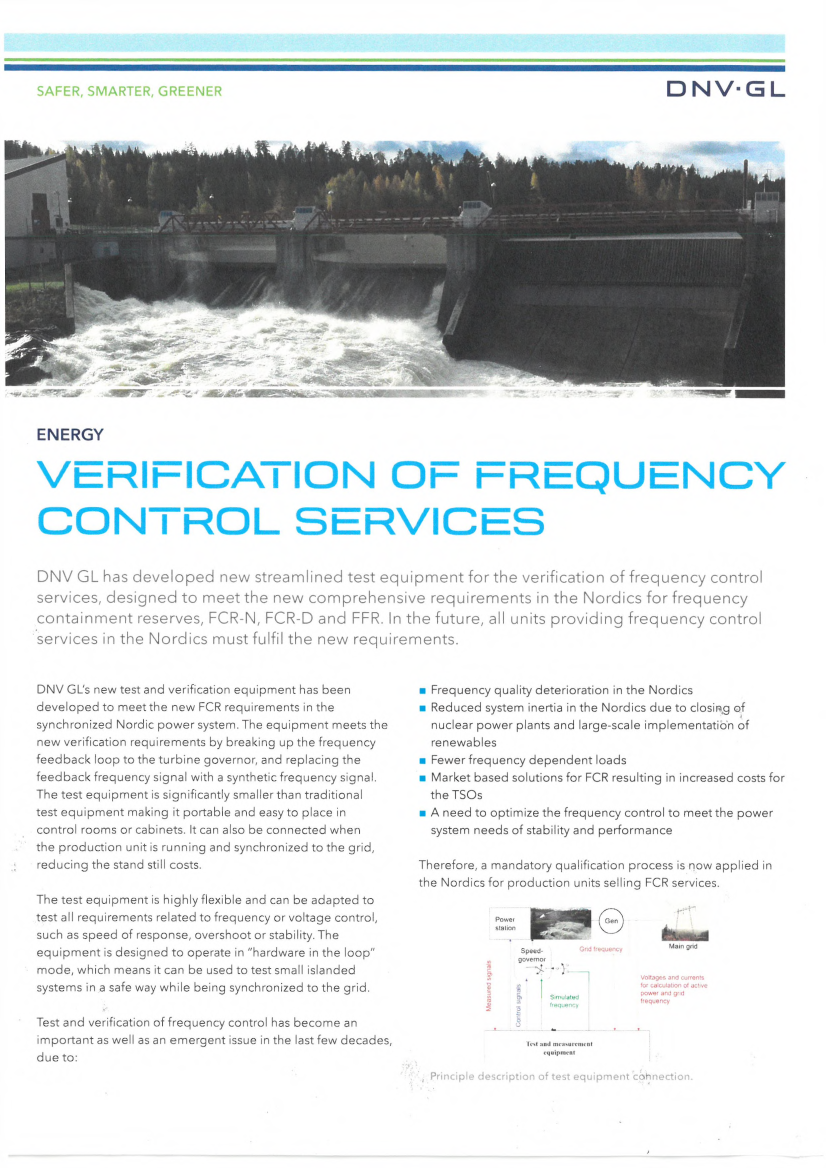
\includegraphics[width=\textwidth]{./pictures/DNV}
						\end{figure}
				\end{column}
		\end{columns}
\end{frame}
\begin{frame}
	\frametitle{Future work}
	\begin{itemize}
			\item Map the market and business potential.
			\item Develop a prototype.
			\item Demonstrate the prototype.
			\item Start a company for testing power plants or sell the idea.
	\end{itemize}
	\end{frame}
